\documentclass[conference]{IEEEtran}

% Keep IEEE's formatting intact. Add packages only when the paper needs them.
\usepackage{cite}
\usepackage{amsmath,amssymb,amsfonts}
\usepackage{graphicx}
\usepackage{textcomp}
\usepackage{xcolor}
\usepackage{listings}

\newcommand{\codefont}{\rmfamily}
\renewcommand{\lstlistingname}{Algorithm}
\lstdefinestyle{pseudocode}{
  basicstyle=\footnotesize\codefont,
  frame=single,
  breaklines=true,
  columns=fullflexible,
  keepspaces=true,
  showstringspaces=false
}

\graphicspath{{figures/}}

\begin{document}

\title{Simulation-Based Evaluation of O-RAN Radio Unit Sleep Policies During Power Outages}

\author{
\IEEEauthorblockN{Sina Shariati}
\IEEEauthorblockA{\textit{Computer Science Department} \\
\textit{University of Twente}\\
Enschede, Netherlands\\
s.shariati-1@student.utwente.nl}
}

\maketitle

\begin{abstract}
Power outages can disable O-RAN radio units (RUs) as their finite local batteries deplete, threatening emergency connectivity when communication is most needed. Operators therefore need to conserve energy without causing service to fall below an emergency target. This study asks how predefined RU sleep policies affect emergency connectivity and RU battery lifetime during a network-wide outage and whether they meet a served-user target of 0.70. It assesses an Always Active (AA) baseline against Staggered Active (SA), which alternates fixed RU groups, and Threshold Staggered Active (TSA), which postpones staggering until all RUs reach a battery threshold. The evaluation compares served-user fraction, horizon-average emergency QoS, mean RU-depletion time, and SLA-based network lifetime within a simplified O-RAN outage model. AA provides the strongest service baseline, with a median SLA-based network lifetime of 21.0 steps. SA lengthens median mean RU-depletion time from 31.2 to 46.2 steps (48\%) but has a median network lifetime of zero. TSA retains near-AA network lifetime (20.5 steps) while extending median mean RU-depletion time to 33.4 steps. Thus, among the fixed policies TSA best preserves target service but modestly extends battery availability, indicating adaptive outage management is needed to make material energy savings without jeopardizing emergency connectivity.
\end{abstract}

\begin{IEEEkeywords}
O-RAN, radio unit, sleep policy, power outage, simulation
\end{IEEEkeywords}


\section{Introduction}

Stable communication is essential during disasters and large-scale power outages, when affected populations and emergency responders depend on cellular networks to obtain and exchange timely information. When grid power is unavailable, radio access networks must rely on finite backup-energy resources to maintain service. In an O-RAN deployment, Radio Unit (RU) operation is therefore critical: an RU that depletes its battery can no longer provide radio access to users within its coverage area~\cite{oranScArchitecture}.

This scenario implies a fundamental trade-off between energy consumption and service availability. Keeping all RUs active maximizes coverage but accelerates battery depletion. In contrast, placing selected RUs into a low-power sleep state conserves energy and extends battery availability, though it may reduce the proportion of users served. Sleep-mode mechanisms are established methods for reducing cellular-network energy consumption \cite{wu2015sleep}; however, during an outage, energy savings alone are insufficient. A policy that preserves battery capacity but does not sustain an acceptable service level cannot be considered dependable for the modeled scenario.

In this work, we study whether simple, predefined RU sleep policies can balance emergency connectivity and battery lifetime during a power outage. Three baseline policies are evaluated: Always Active, in which all RUs remain operational throughout the outage; Staggered Active, where RUs alternate periods of activity; and Threshold Staggered Active, where a predefined threshold determines when RUs rotate their activity. These policies serve as reference points for assessing the trade-offs and limitations of straightforward sleep scheduling. The central research questions are: \emph{How do predefined RU sleep policies influence emergency connectivity and RU battery lifetime in an O-RAN network during a power outage?} \emph{Do these policies meet the configured emergency-service target, or are more adaptive outage-management strategies required?} This work is a controlled, policy-level simulation study rather than a proposal for an optimal scheduling algorithm, a physical-layer-accurate analysis, or a validation of a specific hardware deployment.

This work makes four main contributions:
\begin{itemize}
    \item We formulate a simplified, scenario-specific model of an O-RAN power outage that captures RU battery depletion, active and sleep states, stochastic link quality, capacity-constrained user association, and emergency-service measures.
    \item We conducted controlled simulations of three predefined RU operating policies: Always Active, Staggered Active, and Threshold Staggered Active. The evaluation considers emergency QoS, RU battery-depletion time, and SLA-based network lifetime as complementary measures.
    \item Within the stated model configuration, results show that extending RU battery lifetime does not always ensure reliable emergency service. Periodic staggering maximizes battery extension but often fails to meet the service target early. In contrast, threshold-triggered staggering maintains the service lifetime of the Always Active policy, but offers only a modest battery benefit.
    \item To perform our evaluations, we developed a modular, discrete-time simulation system. This simulator separates policy decisions from the network environment, execution procedure, and metric collection, enabling reproducible comparison of alternative RU control policies.
\end{itemize}

The results show that the battery benefits of predefined sleep policies do not necessarily ensure stable emergency operation. Periodic staggered sleeping achieves the greatest extension of RU battery lifetime but often fails to maintain the configured service target from the start of the outage. Threshold-triggered staggering maintains an SLA-based network lifetime similar to the always-active baseline, yet causes only a modest improvement in battery lifetime. Therefore, under the modeled conditions, the evaluated fixed policies serve as useful reference points but do not provide a sufficiently sound foundation for emergency outage management. Their limitations highlight the need for more adaptive policy designs. This conclusion is specific to the simplified model and experimental configuration employed in this study and does not establish the suitability of these policies for all real-world deployments.

The remainder of this paper is organized as follows. Section~II presents background and related work. Section~III defines the system model and evaluated policies. Section~IV describes the simulation methodology and experimental configuration. Section~V discusses the simulation results, and Section~VI concludes the paper.

\section{Background and Related Work}

Summarize only the background needed to understand the evaluation and position
the paper against existing work.

\subsection{O-RAN Architecture}
Describe the relevant O-RAN components, especially the radio unit and the
control points that could influence energy-aware operation.

\subsection{Radio Unit Energy Resilience}
Explain how radio unit power consumption, backup energy, and outage behavior
affect service continuity.

\subsection{Sleep Strategies}
Review existing radio access network or O-RAN sleep strategies and the
trade-offs they introduce.

\subsection{Gap Addressed}
Identify the specific gap addressed by this comparative simulation-based
evaluation.

\section{System Model and Evaluated Policies}

Define the modeled system and the policies compared in the experiments.

\subsection{Network Model}
Describe the radio units, users, topology, traffic assumptions, and any
abstractions used by the simulator.

\subsection{Outage Assumptions}
Specify outage duration, backup power availability, affected infrastructure,
and recovery assumptions.

\subsection{Connectivity and SINR Model}
Define how user connectivity and signal-to-interference-plus-noise ratio are
computed or approximated.

\subsection{Battery Model}
Describe battery capacity, discharge behavior, sleep-state power consumption,
and active-state power consumption.

\subsection{Emergency QoS Definition}
Define the quality-of-service threshold or service condition used for
emergency connectivity.

\subsection{Evaluated Policies}
Describe each baseline and proposed sleep policy compared in the evaluation.

\section{Simulation Methodology}
\label{sec:simulation-methodology}

We developed an open-source custom discrete-time simulator in Python to evaluate the trade-off between emergency connectivity and RU battery lifetime during power outages. This study analyzes the comparative behavior of predefined RU sleep policies in a controlled, deliberately simplified model. The simulator includes only the mechanisms essential for this comparison: RU battery depletion, active and sleep states, stochastic link quality, user--RU association, and policy-driven state transitions.

Several established platforms for cellular network simulation exist, but they offer capabilities beyond this study's requirements and introduce unnecessary complexity. For example, 5G-LENA and Simu5G support detailed cellular network simulation, while the NIST module models O-RAN-like RIC interactions. The srsRAN project provides a complete 5G CU/DU software stack, and Colosseum, Arena, POWDER, and OpenRAN Gym facilitate emulation and testbed-based experimentation. We did not select these platforms because, to the best of our knowledge, replicating the abstract outage, battery, and association model used in this study would require substantial additional configuration and calibration, without directly benefiting the policy-level comparison. The implemented simulator instead offers a transparent and reproducible environment in which the evaluated policy is the primary experimental variable. This simulator is used exclusively for controlled, policy-level comparisons within the simplified model described in Section~\ref{sec:system-model}. The findings are constrained by the specific assumptions and procedures defined in the study and do not substitute for physical-layer simulation or real-world testing.

The following subsections describe the simulation procedure, experimental configuration, and measurement process.

\subsection{Simulation Architecture and Execution}

The simulator comprises an environment, an RU controller, and metric collectors. The environment maintains the map, RU and user entities, their locations, the connectivity graph, and the current user--RU associations. The controller applies one of the evaluated sleep policies at each timestep. Metric collectors observe the resulting state without influencing the simulation. Figure~\ref{fig:simulator-architecture} depicts the simulator's overall architecture.

\begin{figure*}[t]
    \centering
    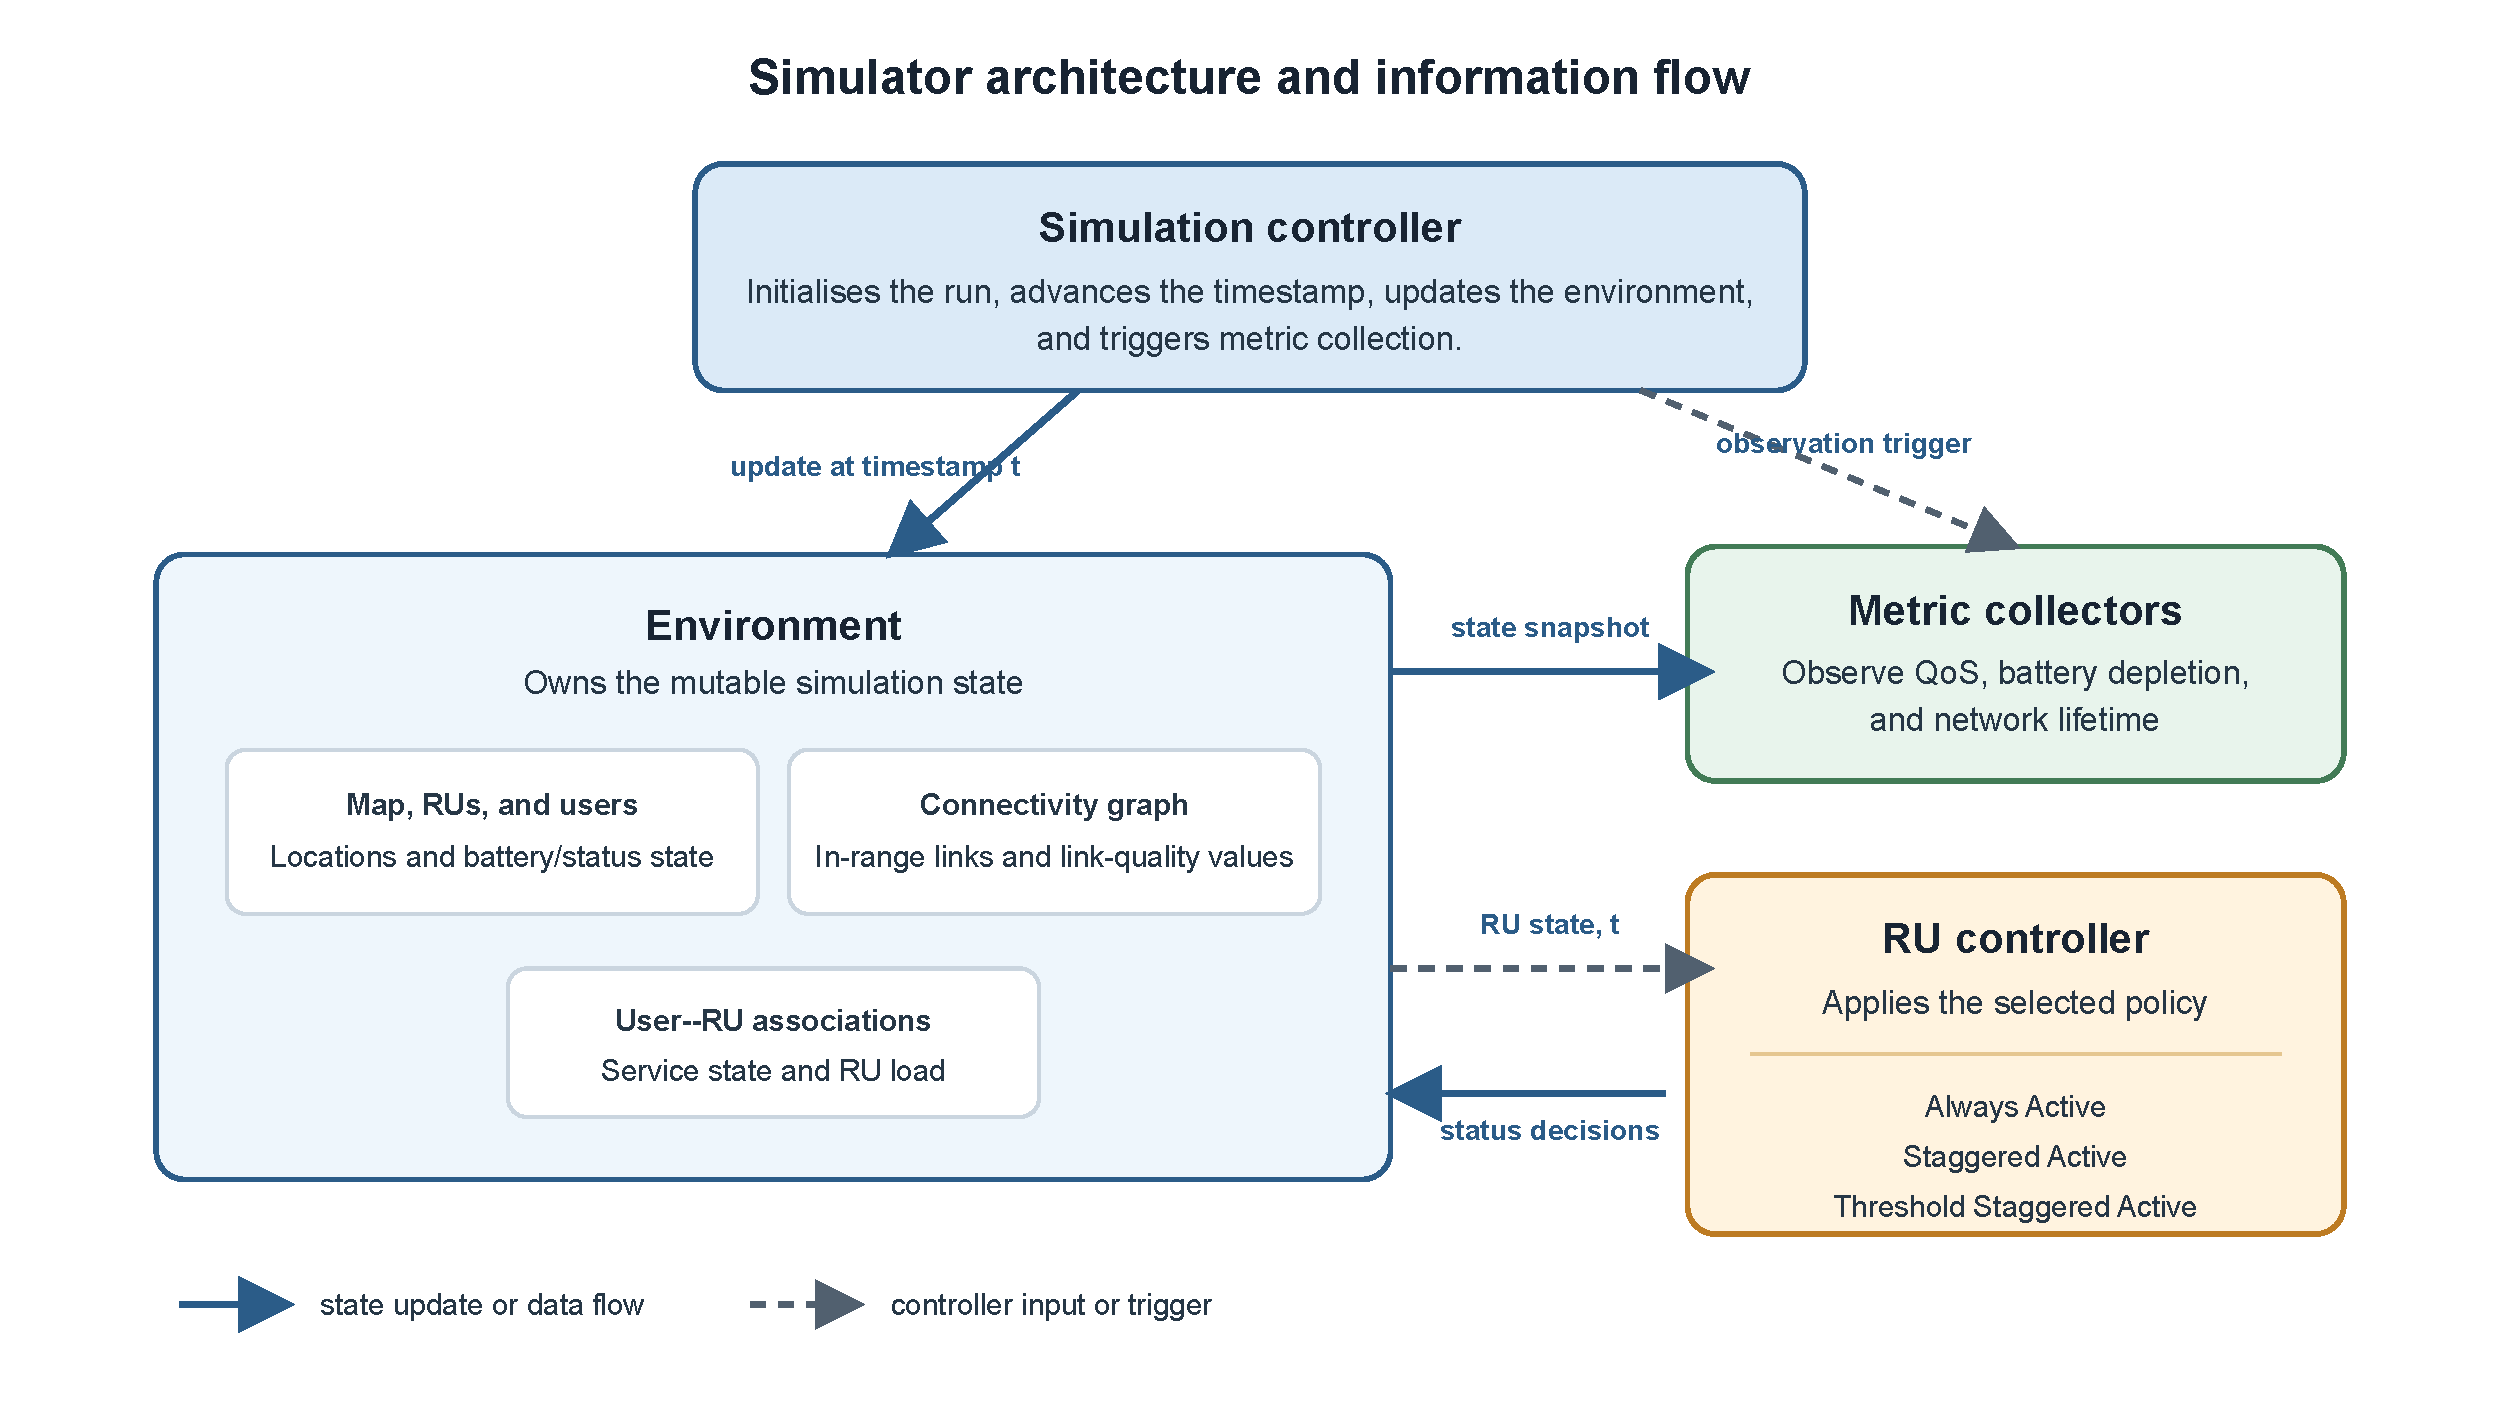
\includegraphics[width=\textwidth]{simulator-architecture}
    \caption{Simulator architecture and information flow. The simulation controller coordinates the environment, RU controller, and metric collectors at each timestep.}
    \label{fig:simulator-architecture}
\end{figure*}

Each simulation run begins at timestamp \(t=0\), when the simulator constructs the environment, generates initial link-quality values, establishes user--RU associations, and records the initial metric observations. The simulation then executes 100 unit-duration timesteps. During each timestep, the simulator first updates RU batteries based on their preceding state and user load. It then applies the selected policy, regenerates link-quality values, recomputes user associations, and records the resulting metrics. This sequence ensures that battery consumption at timestamp \(t\) is determined by the RU state and user associations observed at timestamp \(t-1\), as described in Section~\ref{sec:system-model}.

Algorithm~\ref{alg:simulation-execution} summarizes the simulation control procedure, which calls {\codefont UPDATE\_ENVIRONMENT()} on each timestamp. Moreover, Algorithm~\ref{alg:environment-update} details the {\codefont UPDATE\_ENVIRONMENT()} procedure and connects it to the related formula of the problem model outlined in Section~\ref{sec:system-model}.

\begin{lstlisting}[style=pseudocode, caption={Simulation execution procedure.}, label={alg:simulation-execution}]
procedure RUN_SIMULATION(configuration)
    environment <- BUILD_ENVIRONMENT(configuration)
    controller  <- BUILD_CONTROLLER(configuration.policy)
    collectors  <- BUILD_METRIC_COLLECTORS(configuration.metrics)
    timestamp <- 0

    COLLECT_METRICS(collectors, environment, timestamp)

    for timestamp <- 1 to configuration.simulation_horizon do
        UPDATE_ENVIRONMENT(
            environment,
            controller,
            timestamp,
            configuration.link_quality_threshold
        )
        COLLECT_METRICS(collectors, environment, timestamp)
    end for

    return FINALISE_METRICS(collectors)
end procedure
\end{lstlisting}

\begin{lstlisting}[style=pseudocode, caption={Environment-update procedure.}, label={alg:environment-update}]
procedure UPDATE_ENVIRONMENT(environment, controller, timestamp, threshold)
    for each ru in environment.RUs do
        previous_load <- COUNT_ASSOCIATED_USERS(ru)
        UPDATE_BATTERY(ru, previous_load)
    end for

    controller.UPDATE(environment.RUs, timestamp)

    REGENERATE_LINK_QUALITY(environment)

    associations  <- empty map
    assigned_load <- map each ru to 0
    for each user in SORT_ASCENDING(environment.users, by user_id) do
        candidates <- GET_IN_RANGE_RUS(user, environment)
        candidates <- FILTER_BY_LINK_THRESHOLD(candidates, threshold)
        candidates <- SORT_DESCENDING(candidates, by link_quality)

        for each ru in candidates do
            if ru.status = ACTIVE and
               ru.battery > 0 and
               assigned_load[ru] < ru.user_capacity then
                associations[user] <- ru
                assigned_load[ru] <- assigned_load[ru] + 1
                break
            end if
        end for

        if user not in associations then
            associations[user] <- NONE
        end if
    end for

    environment.associations <- associations
end procedure
\end{lstlisting}

\subsection{Experimental Configuration and Policy Comparison}

Table~\ref{tab:baseline-configuration} summarises the baseline configuration used in every simulation run. The simulation uses a \(20\times20\) discrete grid containing five RUs and thirty users. Entity locations are sampled uniformly without replacement, such that no two entities occupy the same cell. Users and RUs remain stationary for the duration of a run.

\begin{table}[t]
    \caption{Baseline simulation configuration.}
    \label{tab:baseline-configuration}
    \centering
    \footnotesize
    \setlength{\tabcolsep}{3pt}
    \renewcommand{\arraystretch}{1.1}
    \begin{tabular}{p{0.62\columnwidth} p{0.32\columnwidth}}
        \hline
        \textbf{Parameter} & \textbf{Value} \\
        \hline
        Simulation & \(20\times20\) grid cells \\
        Number of RUs & 5 \\
        Number of users & 30 \\
        Initial RU battery & 250 energy units \\
        Initial RU status & Active \\
        Active RU with zero users battery consumption & 1.0 energy units per step \\
        Active RU with one user battery consumption & 2.0 energy units per step \\
        Active RU with two or more users battery consumption & 1.5 energy units per user per step \\
        Sleep consumption & 0.5 energy units per step \\
        RU user capacity & 100 users \\
        Coverage radius & 8 grid cells \\
        Simulation horizon & 100 timesteps \\
        Staggered-policy interval & 10 timesteps \\
        Threshold-policy trigger & 50\% of initial battery \\
        Emergency QoS target & 0.7 \\
        Number of simulation repetitions & 10 \\
        \hline
    \end{tabular}
\end{table}

The time and energy values in Table~\ref{tab:baseline-configuration} are expressed in simulation units. They are not interpreted as seconds, minutes, Joules, or measured hardware power values. This approach enables explicit modeling of energy consumption for policy comparison without implying a direct mapping to a specific RU implementation.

To represent the effect of user load on battery depletion, an active RU incurs a non-zero consumption rate even when it serves no users, because its radio and supporting circuitry must remain powered to maintain availability. Serving the first user is modeled as a transition from an availability-only state to a traffic-bearing state, which introduces additional processing and transmission demand. For two or more served users, the model increases consumption per user in proportion to represent additional scheduling, baseband processing, and transmission activity. The resulting rates therefore distinguish between baseline active operation, the onset of traffic service, and load-dependent energy consumption.

The experiment compares three policies: Always Active, Staggered Active, and Threshold Staggered Active, abbreviated as AA, SA, and TSA, respectively. These policies serve as simple, transparent baselines. AA represents the availability-oriented baseline in which every feasible RU remains active. SA represents a periodic energy-saving strategy in which fixed RU groups alternate between active and sleep states every 10 time steps. TSA represents a hybrid strategy that begins with all feasible RUs active and introduces staggered sleeping only after battery capacities reach the configured threshold. Algorithms~\ref{alg:always-active}, \ref{alg:staggered-active}, and~\ref{alg:threshold-staggered-active} summarize the logic of AA, SA, and TSA policies.

\begin{lstlisting}[style=pseudocode, caption={Always Active policy logic.}, label={alg:always-active}]
procedure ALWAYS_ACTIVE(rus, timestamp)
    for each ru in rus do
        SET_SELECTED_STATUS(ru)
    end for

    return rus
end procedure
\end{lstlisting}

\begin{lstlisting}[style=pseudocode, caption={Staggered Active policy logic.}, label={alg:staggered-active}]
procedure STAGGERED_ACTIVE(rus, timestamp)
    selected_parity <- floor(timestamp / 10) mod 2

    for each ru in rus do
        if ru.id mod 2 = selected_parity then
            SET_SELECTED_STATUS(ru)
        else
            ru.status <- SLEEP
        end if
    end for

    return rus
end procedure
\end{lstlisting}

\begin{lstlisting}[style=pseudocode, caption={Threshold Staggered Active policy logic.}, label={alg:threshold-staggered-active}]
procedure THRESHOLD_STAGGERED_ACTIVE(
    rus,
    timestamp,
    threshold_percentage,
    staggered_started
)

    if rus is empty then
        return rus
    end if

    if not staggered_started then
        threshold_reached <- TRUE

        for each ru in rus do
            battery_percentage <-
                100 * ru.battery / ru.initial_battery

            if battery_percentage > threshold_percentage then
                threshold_reached <- FALSE
                break
            end if
        end for

        if threshold_reached then
            staggered_started <- TRUE
        end if
    end if

    selected_parity <- floor(timestamp / 10) mod 2

    for each ru in rus do
        if not staggered_started then
            SET_SELECTED_STATUS(ru)

        else if ru.id mod 2 = selected_parity then
            SET_SELECTED_STATUS(ru)

        else
            ru.status <- SLEEP
        end if
    end for

    return rus, staggered_started
end procedure
\end{lstlisting}

These policies serve as reference points for assessing whether straightforward sleep scheduling can preserve emergency service while extending battery availability in real-world scenarios. They are not intended as optimal outage-management strategies. Accordingly, the comparison examines the limitations and trade-offs of simple policy logic and assesses whether a more sophisticated policy is necessary.

To increase the generalizability of final results, we conduct multiple simulation repetitions using different seed values. Within each repetition, all three policies use the same seed, ensuring identical RU and user placements and the same sequence of stochastic link-quality values. This paired design reduces the influence of random topology and link variation on the comparison, isolating the selected policy as the intended experimental factor while ensuring the policy is tested across multiple RU and user placements and stochastic link-quality values.

\subsection{Metrics, Analysis Procedure, and Implementation Verification}

As shown in Figure~\ref{fig:simulator-architecture}, the simulator records observations at timestamp \(t=0\) and after each of the 100 timestep updates. The collected metrics are the served-user fraction over time, average emergency QoS, RU battery-depletion time, and network lifetime.

Each policy produces ten final values for every metric, one for each repetition. We retain these values as distributions rather than reducing them immediately to a single mean. Aggregate summaries use medians and interquartile ranges to describe variation between repetitions. The time-series observations similarly support comparison of the typical trajectory and variability of emergency service and RU battery levels across policies.

We verify the implementation through deterministic and behavioral checks. First, identical configurations and random seeds must produce identical simulation outputs. Second, a depleted RU must not serve a user. Third, sleep-state consumption must remain lower than active-state consumption under the configured model. Finally, when all other conditions are unchanged, increasing the initial battery capacity must not reduce the observed battery lifetime. These checks confirm consistency between the implementation and the model defined in Section~\ref{sec:system-model}.

\section{Discussion}

Present the simulation results and interpret what they imply for the research
question.

\subsection{Policy Comparison}
Compare the evaluated policies across the main metrics.

\subsection{Trade-offs}
Explain the trade-offs between energy savings, service availability, and
emergency QoS.

\subsection{Sensitivity Analysis}
Test how results change under important parameter variations.

\subsection{Limitations}
Discuss modeling assumptions, simulator limitations, and external validity.

\subsection{Answer to the Research Question}
State the direct answer supported by the results.

\section{Conclusion}

Concisely summarize the findings, state their implications for outage-resilient
O-RAN operation, and identify realistic future work.

\section*{Generative AI Disclosure}

During the preparation of this work, the authors used generative artificial
intelligence and language-assistance tools, including ChatGPT and Grammarly,
to refine language and augment vocabulary. After using these tools and
services, the authors thoroughly reviewed and edited the content as needed and
take full responsibility for the final outcome.


% References are generated here after cited sources are added.
% \bibliographystyle{ieeetr}
% \bibliography{references}

\end{document}
